\subsection{Aufgabe 1}

Wir sollten die Apparatur aufbauen und justieren. Dabei geht der Strahlengang  des Lichts von der Dampflampe aus durch die Kondensorlinse, in welcher das Licht gesammelt wird. Durch den darauf folgenden Spalt konnte man die Intensität des Lichts regulieren. Die Kollimatorlinse sollte ein möglichst parallelen Strahlengang erzeugen, welcher anschließend zum Prisma gelangt und dort gebrochen wird. Dieser Strahl wird nun durch den Achromator fokussiert, damit nur eine Spektrallinie durch den Spalt vor der Photozelle gelangt. In der Photozelle selbst wird schließlich der Prozess aus Punkt 1.4 in Gang gesetzt.
\\
\begin{center}
\begin{minipage}{\linewidth}
\centering
\makebox[0cm]{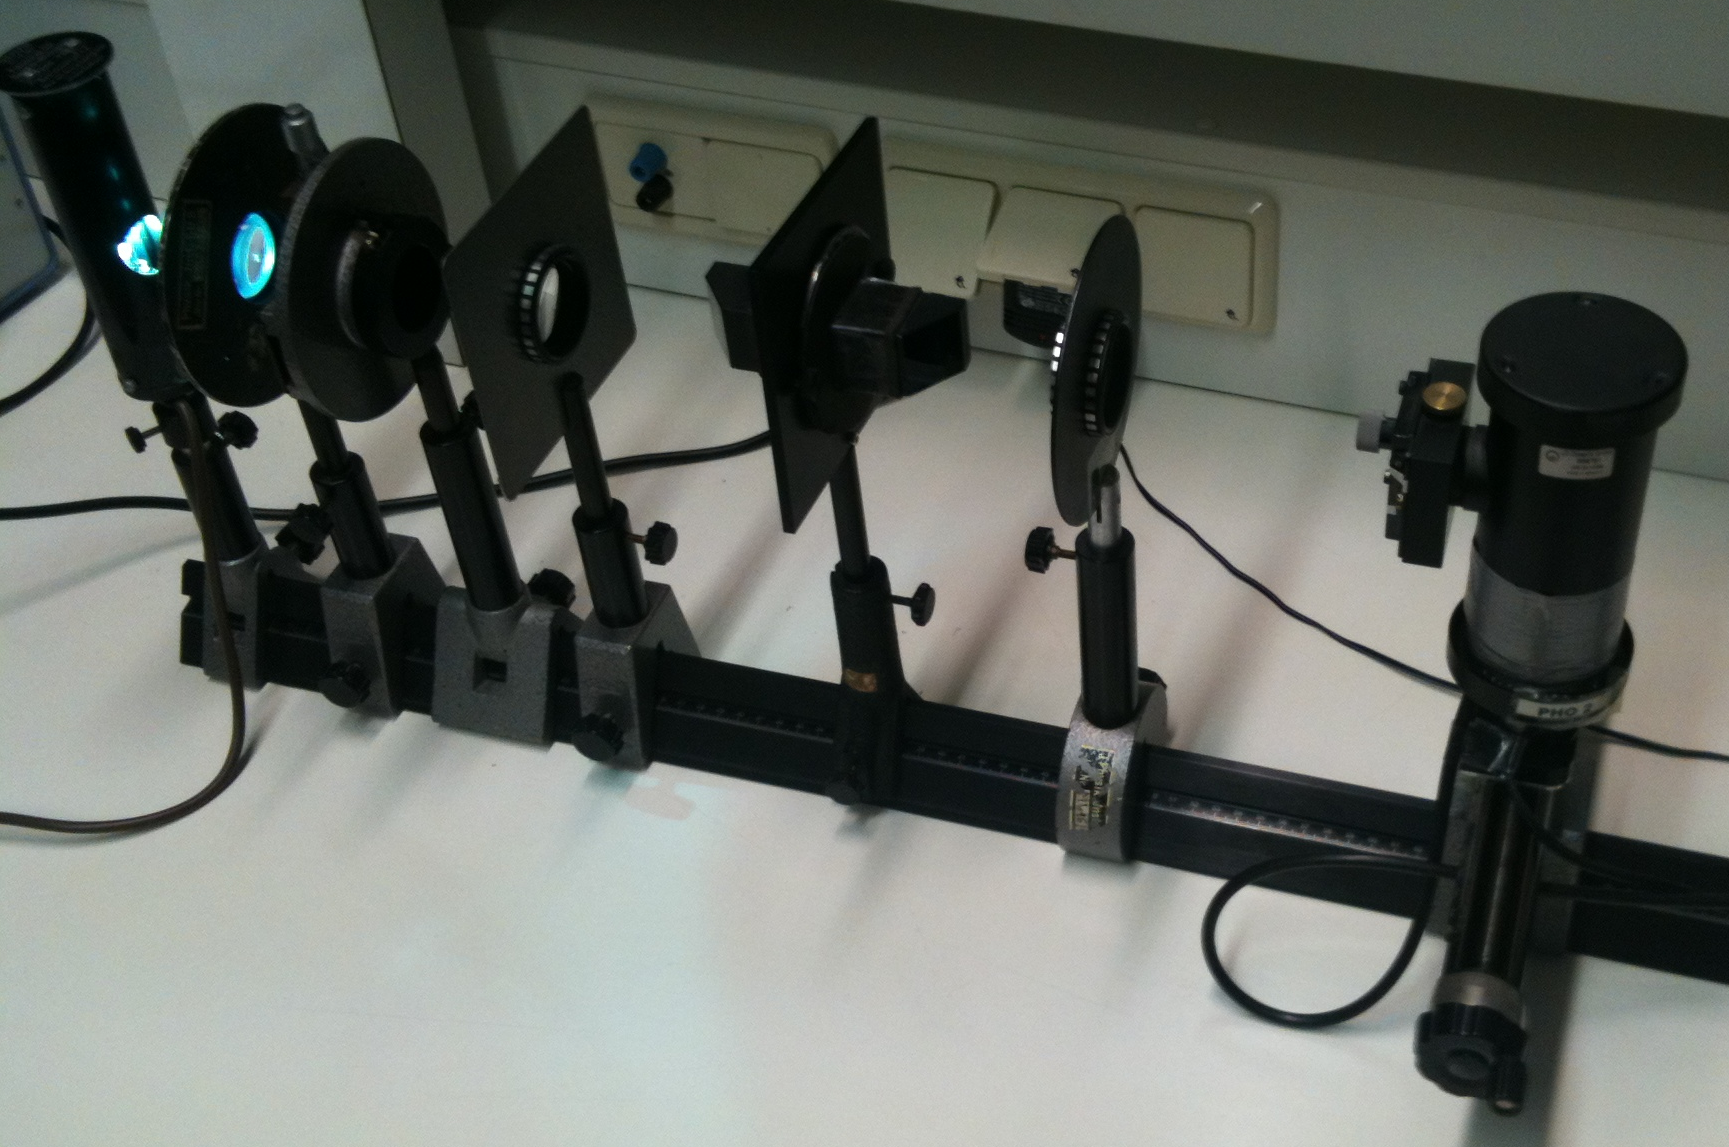
\includegraphics[width=\textwidth]{bilder/pho4}}
\captionof{figure}{Aufbau der Messapparatur (von Links: Hg-Dampflampe, Kondensorlinse, variabler Spalt, Kollimatorlinse, Dispersionsprisma, Achromator, (Kalium-)Photozelle}%
\label{ringe}
\end{minipage}
\end{center}

Beim Justieren hatten wir kleinere Probleme, größtenteils mit der Stromversorgung, wobei wir ein wenig die Positionen der Linsen variierten. Das beeinflusste die gemessenen Testwerte jedoch nicht. Es gibt ansonsten keine Messwerte, Berechnungen und auswertbare Ergebnisse für diese Aufgabe.
\newpage